%%%%%%%%%%%%%%%%%%%%%%%%%%%%%%%%%%%%%%%%%%%%%%%%%%%%%%%%%%%%%%%%%%%%%%%%%%%%%%%%
%%%%%%%%%%%%%%%%%%%%%%%%%%%%%%%%%%%%%%%%%%%%%%%%%%%%%%%%%%%%%%%%%%%%%%%%%%%%%%%%
%\documentclass[addpoints,12pt,solution]{exam}
\documentclass[preprint,12pt]{elsarticle}
%% Use the option review to obtain double line spacing

%% Use the options 1p,twocolumn; 3p; 3p,twocolumn; 5p; or 5p,twocolumn
%% for a journal layout:
%% \documentclass[final,1p,times]{elsarticle}
%% \documentclass[final,1p,times,twocolumn]{elsarticle}
%% \documentclass[final,3p,times]{elsarticle}
%% \documentclass[final,3p,times,twocolumn]{elsarticle}
%% \documentclass[final,5p,times]{elsarticle}
%% \documentclass[final,5p,times,twocolumn]{elsarticle}

%% The graphicx package provides the includegraphics command.
\usepackage{graphicx}
%% The amssymb package provides various useful mathematical symbols
\usepackage{amssymb}
\usepackage{amsmath}
\usepackage{titlesec}
\usepackage{breqn}
\usepackage{chemfig}
\usepackage{csvsimple}
%% The amsthm package provides extended theorem environments
%% \usepackage{amsthm}

%% The lineno packages adds line numbers. Start line numbering with
%% \begin{linenumbers}, end it with \end{linenumbers}. Or switch it on
%% for the whole article with \linenumbers after \end{frontmatter}.
\usepackage{lineno}
\usepackage{natbib}
\usepackage{hyperref}
% \usepackage[top=0.75in, bottom=0.75in, left=0.55in, right=0.85in]{geometry}
\usepackage{graphicx}
\usepackage{url}
\usepackage{palatino}
\usepackage{tabularx}
\usepackage{graphicx}
\usepackage{multicol}
\usepackage{graphicx}
\usepackage{amssymb}
\usepackage{float}
\usepackage{amsmath}
\usepackage{rotating}
\usepackage{subfigure}
\usepackage{multirow}
\usepackage{mathrsfs}
\usepackage{xfrac}
\usepackage[font=small,skip=0pt]{caption}
%\usepackage[numbers,sort&compress]{natbib}
%\usepackage{hyperref}
\usepackage{pgf,tikz}
\usetikzlibrary{shapes,arrows,chains}
\usetikzlibrary[calc]
\usepackage{graphicx}
\graphicspath{ {./images/}}
\usepackage{geometry}
\geometry{lmargin=1in,rmargin=1in,tmargin=1in,bmargin=1in}
\usepackage{lipsum}
%\pagestyle{empty}
\usepackage{natbib}
\pagenumbering{arabic}
%\usepackage[T1]{fontenc}
\usepackage{setspace}
\usepackage{mathptmx}
\usepackage{t1enc}
%\usepackage{xkeyval}
%\usepackage{chemformula}
%\usepackage{array}
%\usepackage{booktabs}
%\usepackage{hypdoc}
%\usepackage{listings}
%\usepackage{lmodern}
%\usepackage{mathpazo}
%\usepackage{microtype}
\usepackage{graphicx}
\usepackage{amssymb}
\usepackage{float}
\usepackage{amsmath}
\usepackage{rotating}
\usepackage{subfigure}
\usepackage{multirow}
\usepackage{xfrac}
\usepackage[font=small,skip=0pt]{caption}
%\usepackage[numbers,sort&compress]{natbib}
%\usepackage{hyperref}
\usepackage{pgf,tikz}
\usetikzlibrary{shapes,arrows,chains}
\usetikzlibrary[calc]
\usepackage{graphicx}
\usepackage{geometry}
\geometry{lmargin=1in,rmargin=1in,tmargin=1in,bmargin=1in}
\usepackage{lipsum}
%\pagestyle{empty}
\usepackage{natbib}
\pagenumbering{arabic}
%\usepackage[T1]{fontenc}
\usepackage{setspace}
\usepackage{mathptmx}
\usepackage{t1enc}
%\usepackage{xkeyval}
%\usepackage{chemformula}
%\usepackage{array}
%\usepackage{booktabs}
%\usepackage{hypdoc}
%\usepackage{listings}
%\usepackage{lmodern}
%\usepackage{mathpazo}
%\usepackage{microtype}
\usepackage{lineno,hyperref}
\usepackage{multirow}
\usepackage{cancel}
\usepackage{url}
\usepackage[norule]{footmisc}
\usepackage[utf8]{inputenc}
\usepackage[english]{babel}
\hypersetup{colorlinks = true,linkcolor = blue,urlcolor = blue}
% \fontfamily{SansSerif}
% \selectfont
% \usepackage[T1]{fontenc}
% \usepackage
%% natbib.sty is loaded by default. However, natbib options can be
%% provided with \biboptions{...} command. Following options are
%% valid:
%%   round  -  round parentheses are used (default)
%%   square -  square brackets are used   [option]
%%   curly  -  curly braces are used      {option}
%%   angle  -  angle brackets are used    <option>
%%   semicolon  -  multiple citations separated by semi-colon
%%   colon  - same as semicolon, an earlier confusion
%%   comma  -  separated by comma
%%   numbers-  selects numerical citations
%%   super  -  numerical citations as superscripts
%%   sort   -  sorts multiple citations according to order in ref. list
%%   sort&compress   -  like sort, but also compresses numerical citations
%%   compress - compresses without sorting
%%
%% \biboptions{comma,round}
% \biboptions{}
\usepackage{caption}
\usepackage{caption}
\usepackage{algorithm} 
\usepackage[noend]{algpseudocode}
\usepackage{amsmath}
\DeclareMathOperator*{\argmin}{argmin}
\DeclareMathOperator*{\argmax}{argmax}
\newcommand*{\argminl}{\argmin\limits}
\newcommand*{\argmaxl}{\argmax\limits}



\begin{document}


\hrule
\vspace{1mm}
\noindent 
\begin{center}
{\Large MA5895 : Numerical Optimization} \\

{\large Combined Assignment Report} \\
{\large Cell Tower Problem   \hfill }
\end{center}
\vspace{1mm}
\noindent 


\titleformat{\section}
{\normalfont\fontfamily{phv}\fontsize{17}{20}\bfseries\itshape}{\thesubsection}{1em}{}

\titleformat{\subsection}
{\normalfont\fontfamily{phv}\fontsize{13}{17}\bfseries\itshape}{\thesubsection}{1em}{}

%%%%%%%%%%%%%%%%%%%%%%%%%%%%%%%%%%%%%%%%%%%%%%%%%%%%%%%%%%%%%%%%
% Enter name and roll number here
\noindent {\bf Name:} Pragnesh Rana \hfill {\bf Roll number:} ME17S301
%%%%%%%%%%%%%%%%%%%%%%%%%%%%%%%%%%%%%%%%%%%%%%%%%%%%%%%%%%%%%%%%%%
\vspace{2mm}
\hrule
\vspace{2mm}
{\small

\textbf{Summary : } Hi

}
\vspace{2mm}
\hrule

%%
%% Following citation commands can be used in the body text:
%% Usage of \cite is as follows:

%%   \cite{key}          ==>>  [#]
%%   \cite[chap. 2]{key} ==>>  [#, chap. 2]
%%   \citet{key}         ==>>  Author [#]

\tableofcontents

\section{Problem Statement}
In city planning, the issue is to place towers for given the population. Divide the population into region based on maximum capacity to plant tower sites. Out of all possible cell tower cites, find out the optimal tower location such that maximum  population is served within limit of budget constrain.




\section{Approach to tackle the problem}

\section{Assumptions}
Assumed that,
\begin{itemize}
	\item The city is a rectangular region
	\item
\end{itemize}


\section{Formulation}
\begin{equation}
V(s) = \argmax_{Q(s,a)} 
\end{equation}

\section{Algorithm}
\section{Results and Discussion}
\subsection{Voronoi Diagram of few values of input}

\begin{figure}[H]
	\centering  
	\subfigure[Grid world with goal G1]
	{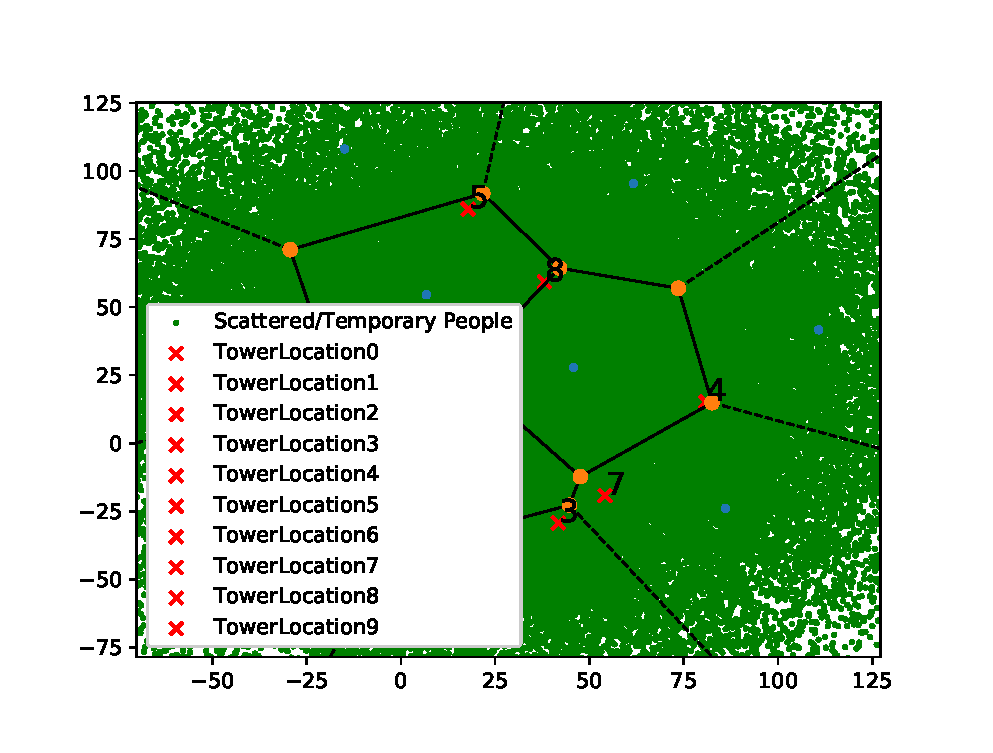
\includegraphics[width=0.43\linewidth]{./FinalResult.eps}\label{grid_a_arrow}}
	\subfigure[Grid world with goal G2]
	{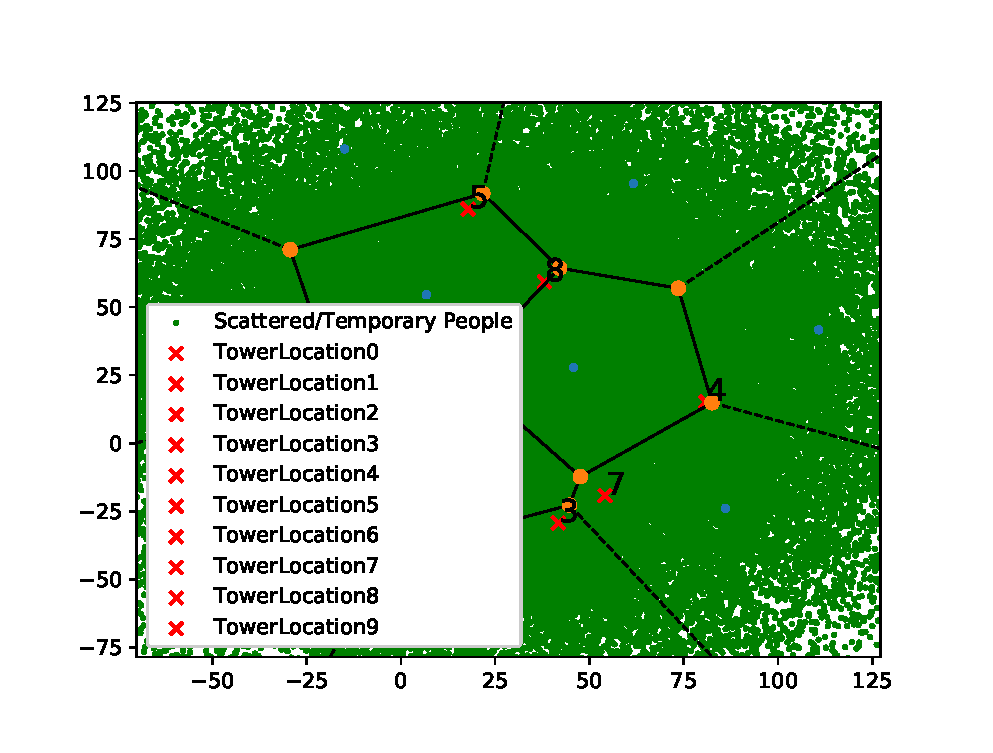
\includegraphics[width=0.43\linewidth]{./FinalResult.eps}\label{grid_b_arrow}}
	\caption{Grid world of four rooms.  Blue:Agent, Green:Terminal The grid world-\ref{grid_a_arrow} has terminal state G1 and grid world-\ref{grid_b_arrow} has terminal state G2. Arrow indicates the optimal policy. The policy in fig-\ref{grid_a_arrow} is obtained using option-1 where as same in fig.-\ref{grid_b_arrow} by option-2 }
	\label{fig:grids}
\end{figure}
\subsection{Computational time as a function of input parameters}
\subsection{Largest problem solution}









	\newpage
	
\section{References}
	%%
	%% Following citation commands can be used in the body text:
	%% Usage of \cite is as follows:
	
	%%   \cite{key}          ==>>  [#]
	%%   \cite[chap. 2]{key} ==>>  [#, chap. 2]
	%%   \citet{key}         ==>>  Author [#]
	
	%% References with bibTeX database:
	\bibliographystyle{ieeetr}
	\bibliography{biblio.bib}					
	%% Authors are advised to submit their bibtex database files. They are
	%% requested to list a bibtex style file in the manuscript if they do
	%% not want to use model1-num-names.bst.
	
	%% References without bibTeX database:
	
	% \begin{thebibliography}{00}
	
	%% \bibitem must have the following form:
	%%   \bibitem{key}...
	%%
	
	% \bibitem{}
	
	% \end{thebibliography}


\end{document}